\documentclass[tikz,border=4pt]{standalone}
\usepackage{amsmath}
\begin{document}
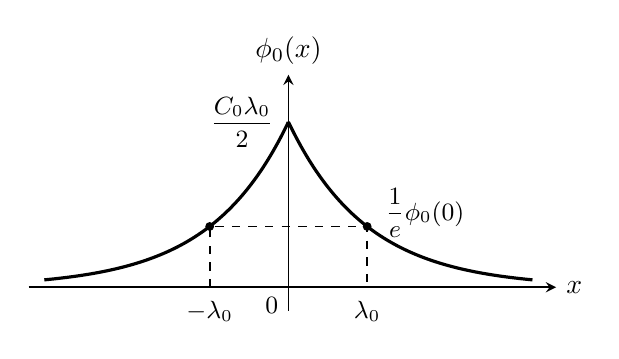
\begin{tikzpicture}[>=stealth, thick, scale=1.0]
  % Axes
  \draw[->, line width=0.65pt] (-3.3, 0) -- (3.4, 0) node[right] {$x$};
  \draw[->, line width=0.65pt] (0, -0.3) -- (0, 2.7) node[above] {$\phi_0(x)$};
  \node[below left, font=\small] at (0, 0) {$0$};

  % Exponential bound-state wavefunction: A * exp(-|x|/lambda_0), A = 2.1, lambda_0 = 1.0
  \draw[line width=1.15pt, domain=0:3.1, samples=80, smooth] plot (\x, {2.1*exp(-\x)});
  \draw[line width=1.15pt, domain=-3.1:0, samples=80, smooth] plot (\x, {2.1*exp(\x)});

  % Mark peak value A = C_0 lambda_0 / 2
  \node[left, font=\small] at (-0.06, 2.1) {$\dfrac{C_0\lambda_0}{2}$};

  % Mark decay length +- lambda_0 at 1/e of peak (y = 2.1 / e = 0.7725)
  \draw[dashed, line width=0.6pt] (-1.0, 0) -- (-1.0, 0.7725) -- (1.0, 0.7725) -- (1.0, 0);
  \fill (-1.0, 0.7725) circle (1.6pt);
  \fill (1.0, 0.7725) circle (1.6pt);
  \node[below, font=\small] at (-1.0, -0.05) {$-\lambda_0$};
  \node[below, font=\small] at (1.0, -0.05) {$\lambda_0$};
  \node[right, font=\small] at (1.1, 0.95) {$\dfrac{1}{e}\phi_0(0)$};
\end{tikzpicture}
\end{document}
